\documentclass[10pt,a4paper]{article}

\usepackage[a4paper, top=0.9cm, bottom=0.9cm, left=1cm, right=1cm]{geometry}
\usepackage{graphicx}
\usepackage{float}
\usepackage{amsmath}
\usepackage{amssymb}
\usepackage{xcolor}
\usepackage{mdframed}
\usepackage{parskip}
\usepackage{enumitem}
\usepackage{titlesec}
\usepackage{booktabs}
\usepackage{array}
\usepackage{tikz}
\usetikzlibrary{arrows.meta, positioning}
\usepackage[T1]{fontenc}

\graphicspath{{../../reference/Network_extracted/figures/Lecture10/}}

\definecolor{keyblue}{RGB}{30, 80, 160}
\definecolor{keybluebg}{RGB}{220, 235, 255}
\definecolor{noteorange}{RGB}{200, 100, 0}
\definecolor{noteorangebg}{RGB}{255, 240, 215}
\definecolor{warnred}{RGB}{180, 30, 30}
\definecolor{warnredbg}{RGB}{255, 220, 220}
\definecolor{defgreen}{RGB}{20, 110, 50}
\definecolor{defgreenbg}{RGB}{215, 245, 225}
\definecolor{headernavy}{RGB}{25, 35, 90}

\newmdenv[linecolor=keyblue,backgroundcolor=keybluebg,linewidth=1.5pt,
  leftline=true,rightline=false,topline=false,bottomline=false,
  innerleftmargin=6pt,innerrightmargin=5pt,
  innertopmargin=2pt,innerbottommargin=2pt,
  skipabove=2pt,skipbelow=2pt]{keybox}

\newmdenv[linecolor=noteorange,backgroundcolor=noteorangebg,linewidth=1.5pt,
  leftline=true,rightline=false,topline=false,bottomline=false,
  innerleftmargin=6pt,innerrightmargin=5pt,
  innertopmargin=2pt,innerbottommargin=2pt,
  skipabove=2pt,skipbelow=2pt]{notebox}

\newmdenv[linecolor=defgreen,backgroundcolor=defgreenbg,linewidth=1.5pt,
  leftline=true,rightline=false,topline=false,bottomline=false,
  innerleftmargin=6pt,innerrightmargin=5pt,
  innertopmargin=2pt,innerbottommargin=2pt,
  skipabove=2pt,skipbelow=2pt]{defbox}

\newmdenv[linecolor=warnred,backgroundcolor=warnredbg,linewidth=1.5pt,
  leftline=true,rightline=false,topline=false,bottomline=false,
  innerleftmargin=6pt,innerrightmargin=5pt,
  innertopmargin=2pt,innerbottommargin=2pt,
  skipabove=2pt,skipbelow=2pt]{warnbox}

\titleformat{\section}[block]{\normalsize\bfseries\color{headernavy}}{}{0pt}{}
  [\vspace{1pt}\rule{\linewidth}{0.6pt}\vspace{1pt}]
\titleformat{\subsection}[block]{\small\bfseries\color{keyblue}}{}{0pt}{}
\titlespacing*{\section}{0pt}{4pt}{1pt}
\titlespacing*{\subsection}{0pt}{2pt}{1pt}

\setlist{nosep, topsep=0pt, itemsep=0pt, leftmargin=1.2em}
\parskip=1pt
\parindent=0pt

% ===========================================================================
\begin{document}
% ===========================================================================

\begin{center}
  {\large\bfseries\color{headernavy} Q8 \textemdash{} Dependability Modeling via Markov Chains}\\[1pt]
  {\small MM10 $\cdot$ Hans-Peter Schwefel}
\end{center}
\vspace{1pt}\hrule height 1pt\vspace{3pt}
For Analysing Dependability, we look at availability and reliability
% ===========================================================================
\section*{1\quad Availability \& Reliability (simple Binary Case)}
% ===========================================================================

\vspace{0pt}
\begin{minipage}[t]{0.38\textwidth}
\vspace{0pt}
\begin{center}
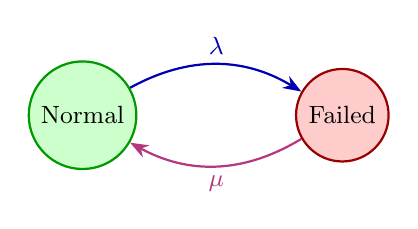
\begin{tikzpicture}[>=Stealth, font=\small]
  \node[draw, circle, minimum size=1.1cm, fill=green!20, draw=green!60!black, line width=0.8pt] (n) {Normal};
  \node[draw, circle, minimum size=1.1cm, fill=red!20, draw=red!60!black, line width=0.8pt, right=2.0cm of n] (f) {Failed};
  \draw[->, blue!70!black, thick] (n) to[bend left=30] node[above, font=\small]{$\lambda$} (f);
  \draw[->, magenta!70!black, thick] (f) to[bend left=30] node[below, font=\small]{$\mu$} (n);
\end{tikzpicture}
\end{center}
\vspace{4pt}
\begin{center}
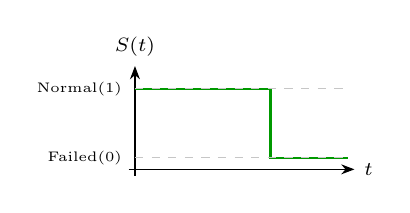
\begin{tikzpicture}[>=Stealth, font=\tiny, scale=0.82]
  \draw[->] (-0.1,0) -- (3.4,0) node[right]{\scriptsize$t$};
  \draw[->] (0,-0.1) -- (0,1.6) node[above]{\scriptsize$S(t)$};
  \node[left, font=\tiny] at (-0.05,1.25) {Normal(1)};
  \node[left, font=\tiny] at (-0.05,0.18) {Failed(0)};
  \draw[green!60!black, thick] (0,1.25) -- (2.1,1.25) -- (2.1,0.18) -- (3.3,0.18);
  \draw[dashed, gray!45, very thin] (0,1.25) -- (3.3,1.25);
  \draw[dashed, gray!45, very thin] (0,0.18) -- (3.3,0.18);
\end{tikzpicture}
\end{center}
\vspace{2pt}
\begin{notebox}
\textcolor{magenta!70!black}{$\mu$} present $\Rightarrow$ \textbf{availability} $A(t)$.\\[2pt]
Remove \textcolor{magenta!70!black}{$\mu$} $\Rightarrow$ \textbf{reliability} $R(t)$: failed absorbing ($Q_\text{red}$).
\end{notebox}
\end{minipage}\hfill
\begin{minipage}[t]{0.59\textwidth}
\vspace{0pt}
\begin{keybox}
\textbf{Availability} --- readiness for correct service:\\[2pt]
$A(t) := \Pr(\text{sys in normal state at time }t)$\\[4pt]
\textbf{Reliability} --- continuity of correct service:\\[2pt]
$R(t) := \Pr(\text{sys in normal state throughout }[0,t])$\\[6pt]
\textit{Assumes exp.\ distributed time-to-failure \& time-to-repair $\Rightarrow$ Markov property (memoryless).}
\end{keybox}
\vspace{2pt}
\begin{warnbox}
\textbf{Key difference:} $A(t)$ uses full $Q$ (repair $\mu$ present). $R(t)$ uses $Q_\text{red}$: failed states absorbing (remove \textcolor{magenta!70!black}{$\mu$} transitions). Only model repair for $A$, not $R$.
\end{warnbox}
\end{minipage}

\vspace{3pt}

% ===========================================================================
\section*{2\quad 2-Component Product State Space Reducant}
% ===========================================================================

\vspace{0pt}
\begin{minipage}[t]{0.46\textwidth}
\vspace{0pt}
\begin{center}
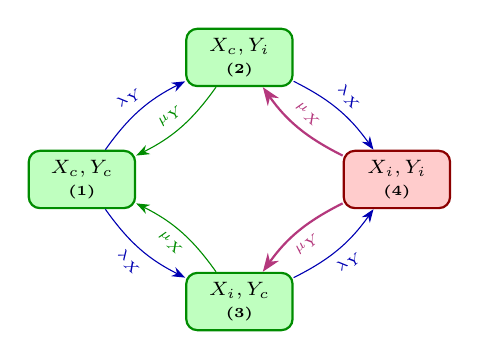
\begin{tikzpicture}[>=Stealth, font=\scriptsize]
  % Diamond layout matching slide: (1)=left, (2)=top, (3)=bottom, (4)=right
  \node[draw, rounded corners, fill=green!25, draw=green!55!black, line width=0.8pt, minimum width=1.35cm, minimum height=0.58cm, align=center]
    (s1) at (-2.0, 0)  {$X_c,Y_c$\\\tiny\textbf{(1)}};
  \node[draw, rounded corners, fill=green!25, draw=green!55!black, line width=0.8pt, minimum width=1.35cm, minimum height=0.58cm, align=center]
    (s2) at (0,  1.55) {$X_c,Y_i$\\\tiny\textbf{(2)}};
  \node[draw, rounded corners, fill=green!25, draw=green!55!black, line width=0.8pt, minimum width=1.35cm, minimum height=0.58cm, align=center]
    (s3) at (0, -1.55) {$X_i,Y_c$\\\tiny\textbf{(3)}};
  \node[draw, rounded corners, fill=red!20, draw=red!55!black, line width=0.8pt, minimum width=1.35cm, minimum height=0.58cm, align=center]
    (s4) at (2.0,  0)  {$X_i,Y_i$\\\tiny\textbf{(4)}};
  % Failure arrows (blue, outside diamond)
  \draw[->, blue!70!black] (s1) to[bend left=14] node[sloped, above, font=\tiny]{$\lambda_Y$} (s2);
  \draw[->, blue!70!black] (s1) to[bend right=14] node[sloped, below, font=\tiny]{$\lambda_X$} (s3);
  \draw[->, blue!70!black] (s2) to[bend left=14] node[sloped, above, font=\tiny]{$\lambda_X$} (s4);
  \draw[->, blue!70!black] (s3) to[bend right=14] node[sloped, below, font=\tiny]{$\lambda_Y$} (s4);
  % Repair 2→1, 3→1 (green, inside diamond, kept in Q_red)
  \draw[->, green!55!black] (s2) to[bend left=14] node[sloped, above, font=\tiny]{$\mu_Y$} (s1);
  \draw[->, green!55!black] (s3) to[bend right=14] node[sloped, below, font=\tiny]{$\mu_X$} (s1);
  % Repair from (4) — magenta, remove for Q_red
  \draw[->, magenta!70!black, thick] (s4) to[bend left=14] node[sloped, above, font=\tiny]{$\mu_X$} (s2);
  \draw[->, magenta!70!black, thick] (s4) to[bend right=14] node[sloped, below, font=\tiny]{$\mu_Y$} (s3);
\end{tikzpicture}
\end{center}
\vspace{1pt}
\begin{notebox}
\textbf{Transistions:}
\begin{itemize}
  \item \textcolor{blue!70!black}{Blue} $\lambda$: failure.
  \item \textcolor{green!55!black}{Green} $\mu$: repair (in $A$ and $R$).
  \item \textcolor{magenta!70!black}{Magenta} $\mu$: \textbf{remove for} $Q_\text{red}$ (state 4 absorbing $\Rightarrow$ reliability).
\end{itemize}
\end{notebox}
\begin{defbox}
\textbf{States:} $c$=correct, $i$=incorrect service.\\
\textcolor{green!55!black}{\textbf{Correct}} $=$ \textcolor{green!55!black}{\textbf{\{1,2,3\}}} ($X_c$ or $Y_c$ still serving).\\
\textcolor{red!65!black}{\textbf{Failed}} $=$ \textcolor{red!65!black}{\textbf{\{4\}}} (both $X_i$ and $Y_i$).
\end{defbox}
\end{minipage}\hfill
\begin{minipage}[t]{0.51\textwidth}
\vspace{0pt}
\begin{keybox}
\textbf{Generator matrix $Q$ ($\lambda$=fail rate, $\mu$=repair rate):}\\[3pt]
$Q\!=\!\left(\begin{matrix}
{-(\lambda_X{+}\lambda_Y)} & \lambda_Y & \lambda_X & 0 \\[2pt]
\mu_Y & {-(\lambda_X{+}\mu_Y)} & 0 & \lambda_X \\[2pt]
\mu_X & 0 & {-(\lambda_Y{+}\mu_X)} & \lambda_Y \\[2pt]
0 & \textcolor{magenta!70!black}{\mu_X} & \textcolor{magenta!70!black}{\mu_Y} & {-(\mu_X{+}\mu_Y)}
\end{matrix}\right)$\\[5pt]
Diagonal $= -\!\sum_\text{outgoing rates}$. Row sums $= 0$.\\[4pt]
\textbf{Transient probabilities:}
\[ \underline{P}(t) = \underline{P}(0)\,\mathrm{expm}(Qt) \]
Matlab: \texttt{P0 * expm(Q*t)}. Start: $\underline{P}(0)=[1,0,0,0]$.\\[4pt]
\textbf{Availability} (redundant): $A(t) = P_1(t)+P_2(t)+P_3(t)$\\[2pt]
\textbf{Reliability}: same but use $Q_\text{red}$: set \textcolor{magenta!70!black}{$\mu_X$, $\mu_Y$ in row 4} $=0$ (state 4 absorbing).\\[4pt]
\textbf{Steady-state:} solve $\underline{\pi}Q=\underline{0}$, $\sum\pi_i=1$.
\end{keybox}
\end{minipage}
\vspace{0.6em}
\begin{notebox}
  \textbf{Note}

  If \textbf{Non-redundant (serial):} correct=\{1\}; failed=\{2,3,4\}.
\end{notebox}

\vspace{3pt}

% ===========================================================================
\section*{3\quad Model Variants}
% ===========================================================================

\vspace{0pt}
\begin{minipage}[t]{0.48\textwidth}
\vspace{0pt}
\begin{keybox}
\textbf{Correlated faults/repairs:}
\begin{itemize}
  \item $X$ fails $\Rightarrow$ $\lambda_Y$ \textbf{increases} in states 2/3
  \item Both fail $(X_i,Y_i)$ $\Rightarrow$ $\mu_X$, $\mu_Y$ \textbf{degrade} (shared technician, slower repair)
\end{itemize}
$\Rightarrow$ Modify $Q$ entries differently per state.
\end{keybox}
\end{minipage}\hfill
\begin{minipage}[t]{0.48\textwidth}
\vspace{0pt}
\begin{defbox}
\textbf{Redundancy variants} (only \emph{active} comp.\ fails):
\begin{itemize}
  \item \textbf{Active standby:} both on $\Rightarrow$ both have $\lambda$
  \item \textbf{On demand (instant):} standby $\lambda{=}0$; switch instant
  \item \textbf{On demand (exp.\ $D$):} add intermediate switching state
\end{itemize}
\textbf{Multiple fault types} (HW + SW): rates add: $\lambda{=}\lambda_{hw}{+}\lambda_{sw}$. Repair destination/rate depends on fault type.
\end{defbox}
\end{minipage}

\clearpage

% ===========================================================================
\section*{4\quad Non-Constant Failure Rates: Bathtub Model}
% ===========================================================================

\vspace{0pt}
\begin{minipage}[t]{0.42\textwidth}
\vspace{0pt}
\begin{center}
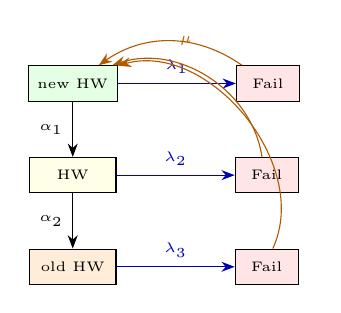
\begin{tikzpicture}[>=Stealth, font=\tiny, node distance=0.2cm]
  \node[draw, fill=green!10, minimum width=1.1cm, minimum height=0.45cm, align=center] (w1) {new HW};
  \node[draw, fill=red!10, minimum width=0.8cm, minimum height=0.45cm, align=center, right=1.5cm of w1] (f1) {Fail};
  \node[draw, fill=yellow!10, minimum width=1.1cm, minimum height=0.45cm, align=center, below=0.7cm of w1] (w2) {HW};
  \node[draw, fill=red!10, minimum width=0.8cm, minimum height=0.45cm, align=center, right=1.5cm of w2] (f2) {Fail};
  \node[draw, fill=orange!15, minimum width=1.1cm, minimum height=0.45cm, align=center, below=0.7cm of w2] (w3) {old HW};
  \node[draw, fill=red!10, minimum width=0.8cm, minimum height=0.45cm, align=center, right=1.5cm of w3] (f3) {Fail};
  % Aging transitions
  \draw[->] (w1) -- node[left, font=\tiny]{$\alpha_1$} (w2);
  \draw[->] (w2) -- node[left, font=\tiny]{$\alpha_2$} (w3);
  % Failure rates
  \draw[->, blue!70!black] (w1) -- node[above, font=\tiny]{$\lambda_1$} (f1);
  \draw[->, blue!70!black] (w2) -- node[above, font=\tiny]{$\lambda_2$} (f2);
  \draw[->, blue!70!black] (w3) -- node[above, font=\tiny]{$\lambda_3$} (f3);
  % Repair → new HW (orange, technician replaces)
  \draw[->, orange!70!black] (f1) to[bend right=35] node[right, font=\tiny]{$\mu$} (w1);
  \draw[->, orange!70!black] (f2) to[bend right=50] (w1);
  \draw[->, orange!70!black] (f3) to[bend right=65] (w1);
\end{tikzpicture}
\end{center}
\end{minipage}\hfill
\begin{minipage}[t]{0.55\textwidth}
\vspace{0pt}
\begin{keybox}
\small\textbf{Bathtub hazard rate:} $\lambda_1 > \lambda_2 < \lambda_3$
\begin{itemize}
  \item $\lambda_1$ high: early life (production errors)
  \item $\lambda_2$ low: useful life
  \item $\lambda_3$ high: wear-out / aging
\end{itemize}
Model: 3 HW-quality states each with matching Fail state = 6-state CTMC. Aging: $\alpha_1$, $\alpha_2$ transitions (working states degrade over time).
\end{keybox}
\vspace{2pt}
\begin{notebox}
\small\textbf{Repair depends on model:}\\
\textbf{New HW} (orange): technician replaces $\Rightarrow$ $\mu$ returns to \emph{new HW} state (same $\lambda$ as brand new).\\
\textbf{Fix only}: returns to same HW phase (may also include $\mu$ for HW replacement). $\mu$ rate and destination depend on what is modelled.
\end{notebox}
\end{minipage}

\vspace{4pt}

% ===========================================================================
\section*{5\quad TMR: Triple Module Redundancy}
% ===========================================================================

\vspace{0pt}
\begin{minipage}[t]{0.36\textwidth}
\vspace{0pt}
\begin{center}
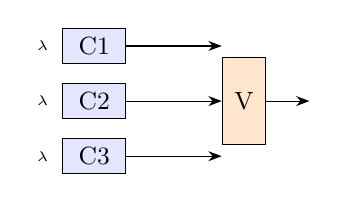
\begin{tikzpicture}[>=Stealth, font=\small, node distance=0.3cm]
  \node[draw, fill=blue!10, minimum width=0.8cm, minimum height=0.4cm] (c1) at (0,0.7) {C1};
  \node[draw, fill=blue!10, minimum width=0.8cm, minimum height=0.4cm] (c2) at (0,0) {C2};
  \node[draw, fill=blue!10, minimum width=0.8cm, minimum height=0.4cm] (c3) at (0,-0.7) {C3};
  \node[draw, fill=orange!20, minimum width=0.55cm, minimum height=1.1cm, align=center] (v) at (1.9,0) {\small V};
  \draw[->] (c1.east) -- (v.west|-c1.east);
  \draw[->] (c2.east) -- (v.west);
  \draw[->] (c3.east) -- (v.west|-c3.east);
  \draw[->] (v.east) -- ++(0.55,0);
  \node[left=0.05cm of c1, font=\tiny] {$\lambda$};
  \node[left=0.05cm of c2, font=\tiny] {$\lambda$};
  \node[left=0.05cm of c3, font=\tiny] {$\lambda$};
\end{tikzpicture}
\end{center}
\end{minipage}\hfill
\begin{minipage}[t]{0.61\textwidth}
\vspace{0pt}
\begin{keybox}
\small``2-out-of-3'' with perfect voter (system works if $\geq 2$ of 3 OK):
\[ R(t) = 3R_c(t)^2 - 2R_c(t)^3, \quad R_c(t) = e^{-\lambda t} \]
\[ \mathrm{MTTF}_c = \tfrac{1}{\lambda} \quad\text{vs.}\quad \mathrm{MTTF}_\text{TMR} = \tfrac{5}{6\lambda} \]
\end{keybox}
\vspace{2pt}
\begin{warnbox}
\small\textbf{TMR:} lower MTTF than single component, but \textbf{higher $R(t)$ short-term} $\Rightarrow$ useful for short mission times.\\[2pt]
\textbf{Warning:} MTTF alone does not fully characterise dependability --- it says nothing about the distribution shape (single-component MTTF $>$ TMR MTTF, yet TMR is more reliable early on).
\end{warnbox}
\end{minipage}

\end{document}
